\chapter{ElegantBook 写作示例}

\begin{introduction}
  \item 积分定义~\ref{def:int}
  \item Fubini 定理~\ref{thm:fubi}
  \item 最优性原理~\ref{pro:max}
  \item 柯西列性质~\ref{property:cauchy}
  \item 韦达定理
\end{introduction}

\section{Lebesgue 积分}
在前面各章做了必要的准备后,本章开始介绍新的积分。在 Lebesgue 测度理论的基础上建立了 Lebesgue 积分,其被积函数和积分域更一般,可以对有界函数和无界函数统一处理。正是由于 Lebesgue 积分的这些特点,使得 Lebesgue 积分比 Riemann 积分具有在更一般条件下的极限定理和累次积分交换积分顺序的定理,这使得 Lebesgue 积分不仅在理论上更完善,而且在计算上更灵活有效。

Lebesgue 积分有几种不同的定义方式。我们将采用逐步定义非负简单函数,非负可测函数和一般可测函数积分的方式。

由于现代数学的许多分支如概率论、泛函分析、调和分析等常常用到一般空间上的测度与积分理论,在本章最后一节将介绍一般的测度空间上的积分。

\subsection{积分的定义}

我们将通过三个步骤定义可测函数的积分。首先定义非负简单函数的积分。以下设 $E$ 是 $\mathcal{R}^n$ 中的可测集。

\begin{definition}[可积性] \label{def:int} 
设 $ f(x)=\sum\limits_{i=1}^{k} a_i \chi_{A_i}(x)$ 是 $E$ 上的\textbf{非负简单函数},中文其中 $\{A_1,A_2,\ldots,A_k\}$ 是 $E$ 上的一个可测分割,$a_1,a_2,\ldots,a_k$ 是非负实数。定义 $f$ 在 $E$ 上的积分为 $\int_{a}^b f(x)$
\begin{equation}
   \label{inter}
   \int_{E} f dx = \sum_{i=1}^k a_i m(A_i) \pi \alpha\beta\sigma\gamma\nu\xi\epsilon\varepsilon. \oint_{a}^b\ointop_{a}^b\prod_{i=1}^n
\end{equation}
一般情况下 $0 \leq \int_{E} f dx \leq \infty$。若 $\int_{E} f dx < \infty$,则称 $f$ 在 $E$ 上可积。
\end{definition}

一个自然的问题是,Lebesgue 积分与我们所熟悉的 Riemann 积分有什么联系和区别?在 4.4 在我们将详细讨论 Riemann 积分与 Lebesgue 积分的关系。这里只看一个简单的例子。设 $D(x)$ 是区间 $[0,1]$ 上的 Dirichlet 函数。即 $D(x)=\chi_{Q_0}(x)$,其中 $Q_0$ 表示 $[0,1]$ 中的有理数的全体。根据非负简单函数积分的定义,$D(x)$ 在 $[0,1]$ 上的 Lebesgue 积分为
\begin{equation}
   \label{inter2}
   \int_0^1 D(x)dx = \int_0^1 \chi_{Q_0} (x) dx = m(Q_0) = 0
\end{equation}
即 $D(x)$ 在 $[0,1]$ 上是 Lebesgue 可积的并且积分值为零。但 $D(x)$ 在 $[0,1]$ 上不是 Riemann 可积的。


有界变差函数是与单调函数有密切联系的一类函数。有界变差函数可以表示为两个单调递增函数之差。与单调函数一样,有界变差函数几乎处处可导。与单调函数不同,有界变差函数类对线性运算是封闭的,它们构成一线空间。练习题 \ref{exer:43} 是一个性质的证明。

\begin{exercise}\label{exer:43}
设 $f \notin\in L(\mathcal{R}^1)$,$g$ 是 $\mathcal{R}^1$ 上的有界可测函数。证明函数
\begin{equation}
   \label{ex:1}
   I(t) = \int_{\mathcal{R}^1} f(x+t)g(x)dx \quad t \in \mathcal{R}^1
\end{equation}
是 $\mathcal{R}^1$ 上的连续函数。 
\end{exercise}

\begin{solution}
即 $D(x)$ 在 $[0,1]$ 上是 Lebesgue 可积的并且积分值为零。但 $D(x)$ 在 $[0,1]$ 上不是 Riemann 可积的。
\end{solution}

\begin{proof}
即 $D(x)$ 在 $[0,1]$ 上是 Lebesgue 可积的并且积分值为零。但 $D(x)$ 在 $[0,1]$ 上不是 Riemann 可积的。
\end{proof}

\begin{theorem}[Fubini 定理] \label{thm:fubi} 
(1)若 $f(x,y)$ 是 $\mathcal{R}^p\times\mathcal{R}^q$ 上的非负可测函数,则对几乎处处的 $x\in \mathcal{R}^p$,$f(x,y)$ 作为 $y$ 的函数是 $\mathcal{R}^q$ 上的非负可测函数,$g(x)=\int_{\mathcal{R}^q}f(x,y) dy$ 是 $\mathcal{R}^p$ 上的非负可测函数。并且
\begin{equation}
   \label{eq:461}
   \int_{\mathcal{R}^p\times\mathcal{R}^q} f(x,y) dxdy=\int_{\mathcal{R}^p}\left(\int_{\mathcal{R}^q}f(x,y)dy\right)dx.
\end{equation}

(2)若 $f(x,y)$ 是 $\mathcal{R}^p\times\mathcal{R}^q$ 上的可积函数,则对几乎处处的 $x\in\mathcal{R}^p$,$f(x,y)$ 作为 $y$ 的函数是 $\mathcal{R}^q$ 上的可积函数,并且 $g(x)=\int_{\mathcal{R}^q}f(x,y) dy$ 是 $\mathcal{R}^p$ 上的可积函数。而且~\ref{eq:461} 成立。
\end{theorem}

\ref{thm:fubi}

\begin{note}
在本模板中,引理(lemma),推论(corollary)的样式和定理~\ref{thm:fubi} 的样式一致,包括颜色,仅仅只有计数器的设置不一样。
\end{note}

我们说一个实变或者复变量的实值或者复值函数是在区间上平方可积的,如果其绝对值的平方在该区间上的积分是有限的。所有在勒贝格积分意义下平方可积的可测函数构成一个希尔伯特空间,也就是所谓的 $L^2$ 空间,几乎处处相等的函数归为同一等价类。形式上,$L^2$ 是平方可积函数的空间和几乎处处为 0 的函数空间的商空间。

\begin{proposition}[最优性原理] \label{pro:max}
如果 $u^*$ 在 $[s,T]$ 上为最优解,则 $u^*$ 在 $[s, T]$ 任意子区间都是最优解,假设区间为 $[t_0, t_1]$ 的最优解为 $u^*$ ,则 $u(t_0)=u^{*}(t_0)$,即初始条件必须还是在 $u^*$ 上。
\end{proposition}

我们知道最小二乘法可以用来处理一组数据,可以从一组测定的数据中寻求变量之间的依赖关系,这种函数关系称为经验公式。本课题将介绍最小二乘法的精确定义及如何寻求点与点之间近似成线性关系时的经验公式。假定实验测得变量之间的 $n$ 个数据,则在平面上,可以得到 $n$ 个点,这种图形称为 “散点图”,从图中可以粗略看出这些点大致散落在某直线近旁, 我们认为其近似为一线性函数,下面介绍求解步骤。

\begin{figure}[htbp]
  \centering
  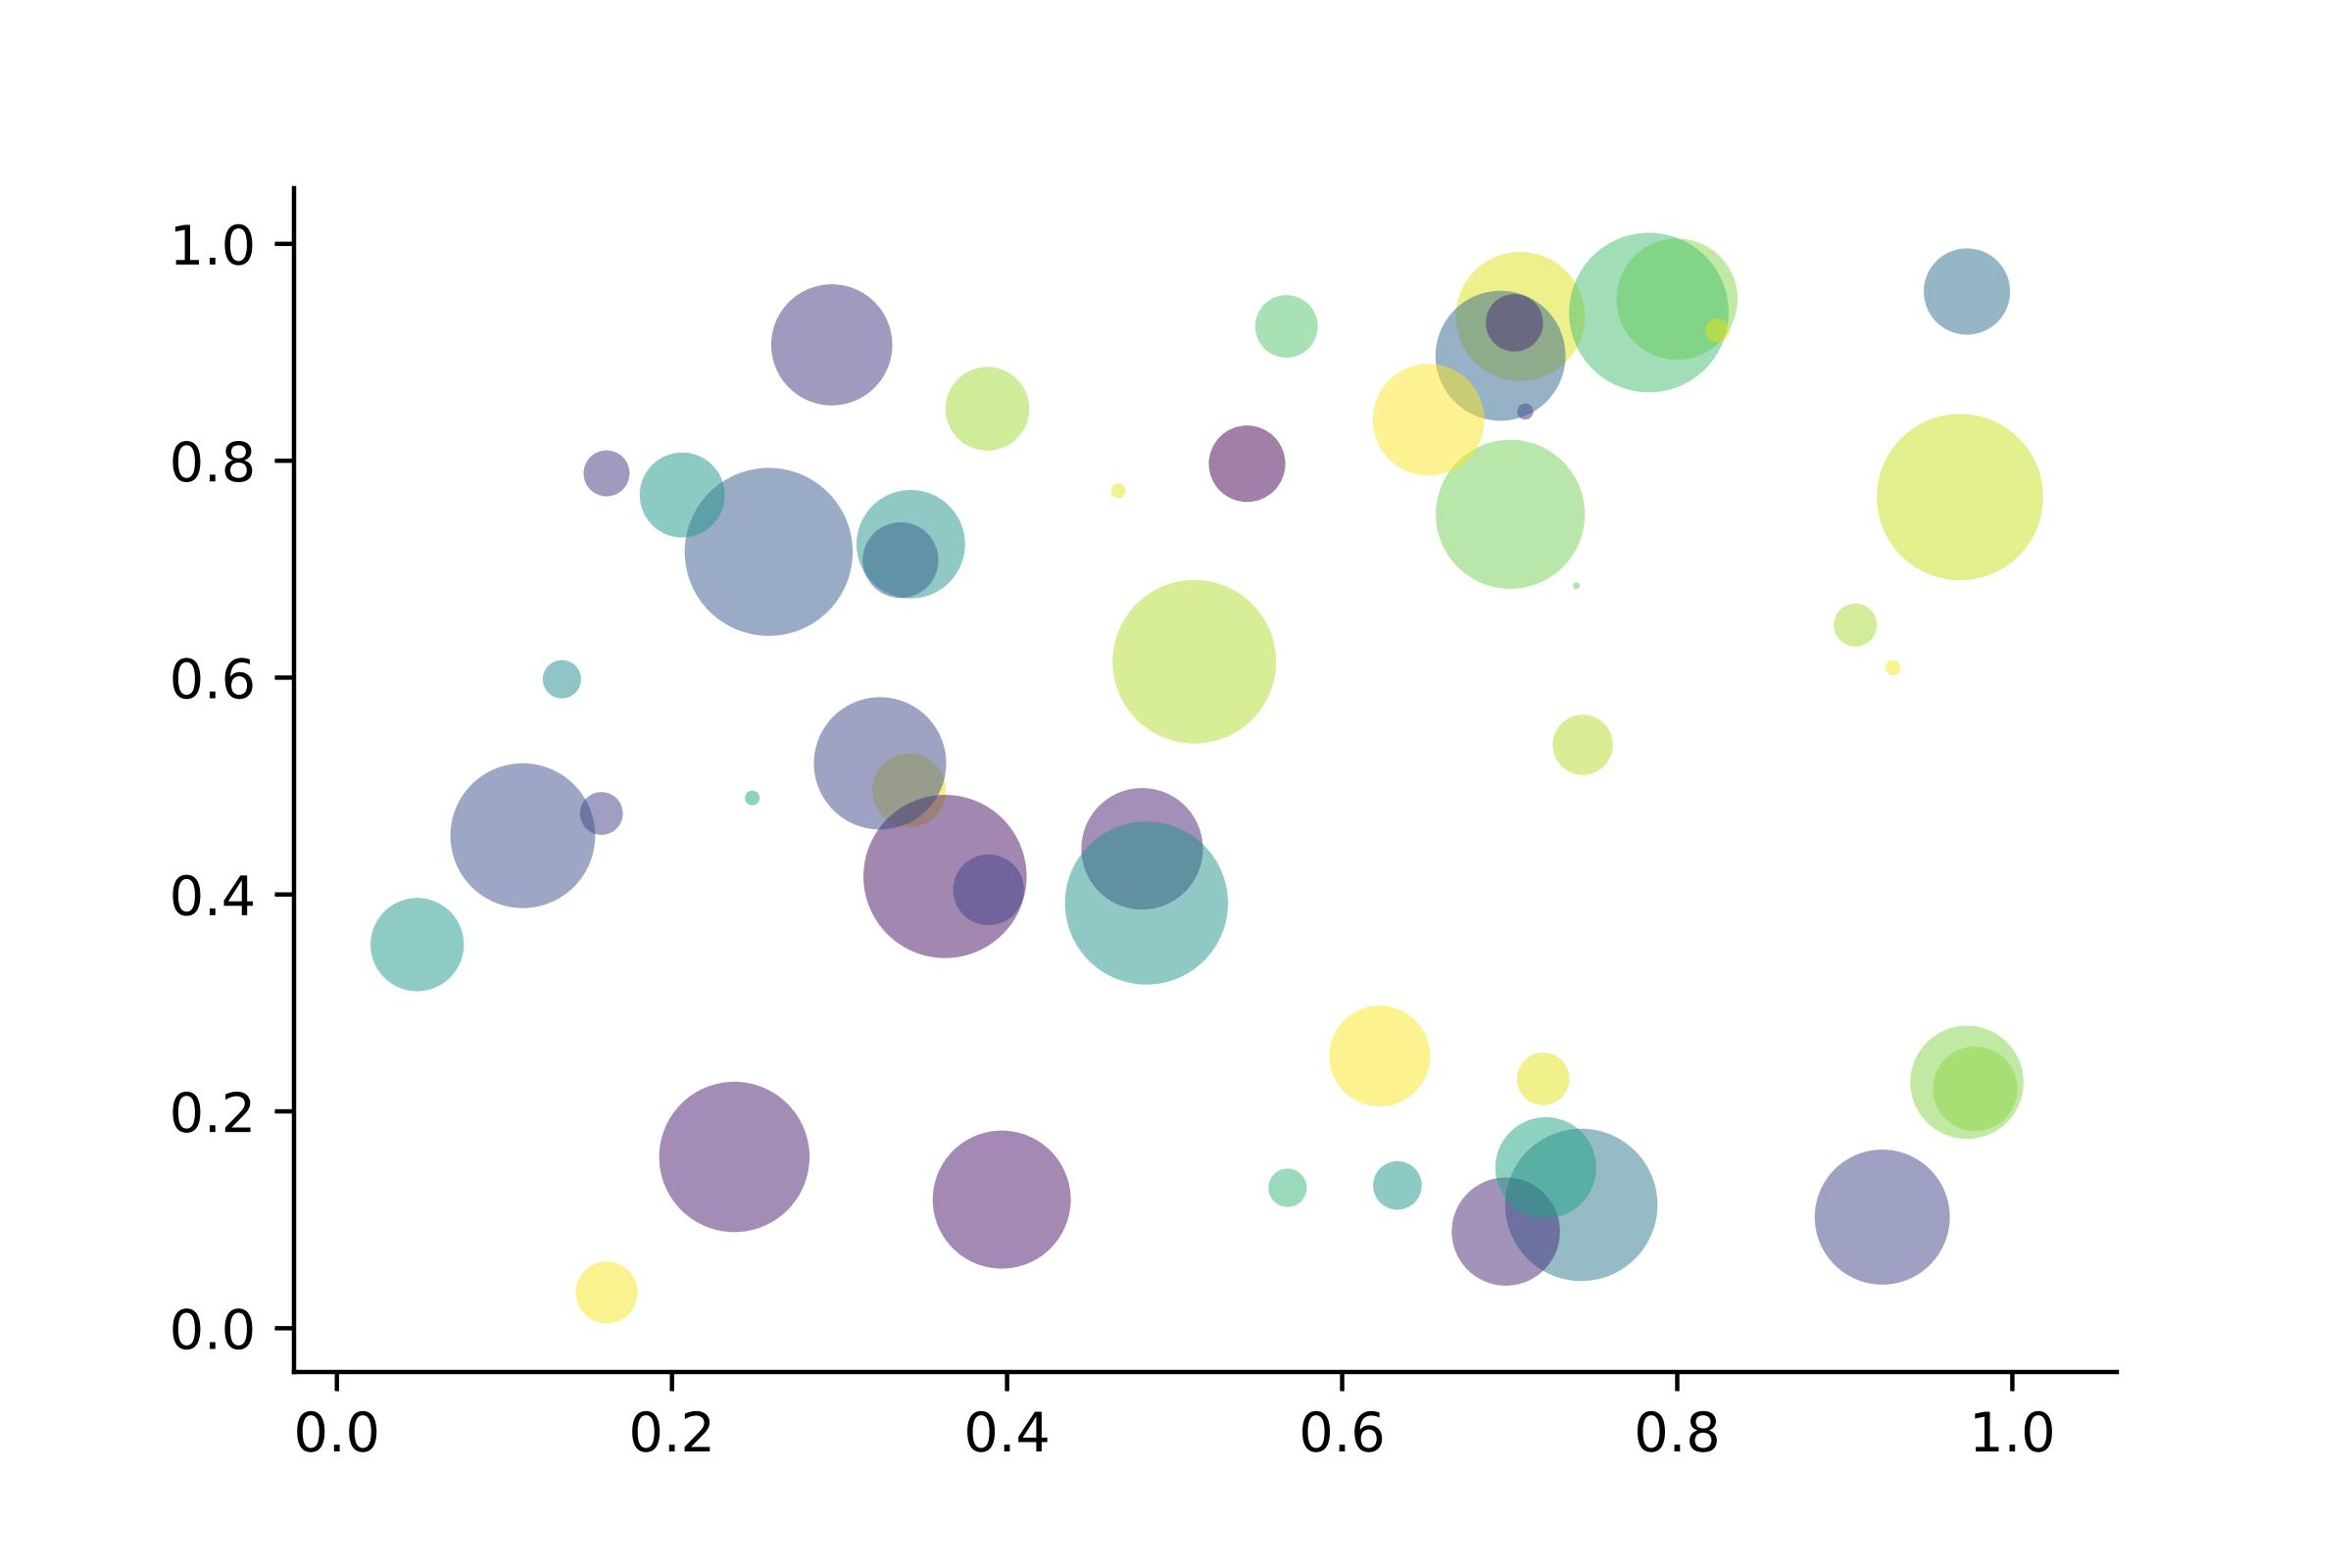
\includegraphics[width=0.6\textwidth]{scatter.jpg}
  \caption{散点图示例 $\hat{y}=a+bx$ \label{fig:scatter}}
\end{figure}

以最简单的一元线性模型来解释最小二乘法。什么是一元线性模型呢?监督学习中,如果预测的变量是离散的,我们称其为分类(如决策树,支持向量机等),如果预测的变量是连续的,我们称其为回归。回归分析中,如果只包括一个自变量和一个因变量,且二者的关系可用一条直线近似表示,这种回归分析称为一元线性回归分析。如果回归分析中包括两个或两个以上的自变量,且因变量和自变量之间是线性关系,则称为多元线性回归分析。对于二维空间线性是一条直线;对于三维空间线性是一个平面,对于多维空间线性是一个超平面。

\begin{property}\label{property:cauchy}
柯西列的性质
\begin{enumerate}
\item $\{x_k\}$ 是柯西列,则其子列 $\{x_k^i\}$ 也是柯西列。
\item $x_k\in \mathcal{R}^n$,$\rho(x,y)$ 是欧几里得空间,则柯西列收敛,$(\mathcal{R}^n,\rho)$ 空间是完备的。
\end{enumerate}
\end{property}

\begin{conclusion}
回归分析(regression analysis) 是确定两种或两种以上变量间相互依赖的定量关系的一种统计分析方法。运用十分广泛,回归分析按照涉及的变量的多少,分为一元回归和多元回归分析;按照因变量的多少,可分为简单回归分析和多重回归分析;按照自变量和因变量之间的关系类型,可分为线性回归分析和非线性回归分析。
\end{conclusion}

\begin{problemset}
\item 设 $A$ 为数域 $K$ 上的 $n$ 级矩阵。证明:如果 $K^n$ 中任意非零列向量都是 $A$ 的特征向量,则 $A$ 一定是数量矩阵。
\item 证明:不为零矩阵的幂零矩阵不能对角化。
\item 设 $A = (a_{ij})$ 是数域 $K$ 上的一个 $n$ 级上三角矩阵,证明:如果 $a_{11} = a_{22} = \cdots = a_{nn}$,并且至少有一个 $a_{kl} \not = 0 (k < l)$,则 $A$ 一定不能对角化。
\end{problemset}

